\chapter{Vertikale Evolution} % 13 Seiten
Dieses Kapitel betrachtet die vertikale Evolution der agilen Softwareentwicklung. Wie bereits erörtert, befinden sich Vorgehensweisen und Prozesse in einem stetigen Wandel. Agile Vorgehensweisen haben viele Probleme der Softwareentwicklung bereits gelöst, sind jedoch nur auf diesen Bereich beschränkt. DevOps hingegen umfasst einige weitere Ebenen, wodurch sich deutlich umfangreichere Möglichkeiten ergeben. Diese werden nachfolgend betrachtet.


\section{Abgrenzung zu Lean und Agile} % 1 Seite
Neben DevOps besteht noch eine Vielzahl an weiteren Prozessen und Vorgehensweisen, welche verwandt, aufbauend, oder vollkommen eigenständig sind. Zwei der am weitest verbreiteten sind agile Entwicklung und Lean. Beide werden oft im Zusammenhang mit DevOps genannt. Manchmal werden diese jedoch fälschlicherweise synonym verwendet. Daher erfolgt zuerst eine Abgrenzung zu diesen beiden Vorgehensweisen.

\subsection{Lean}
Die Lean Bewegung, geprägt von Eric Ries und dessen Buch \glqq The Lean Startup\grqq, verfolgt die Idee, der Prozessoptimierung und Konzentration auf Kernideen. Hierbei wird versucht, den Prozess von der Idee, über Ausarbeitung und Testing, hin zum fertigen Feature möglichst schlank und ressourcenschonend zu halten. Dies ist besonders im Start Up Umfeld sehr interessant, da dort finanzielle Mittle meist recht knapp bemessen sind und die Produkte noch nicht genau definiert sind. Mit Hilfe von Lean kann frühzeitig Kundenfeedback eingeholt werden, was die Entwicklung des Produkts und die Definition eines Zielmarkts deutlich vereinfacht.\\
Lean verfolgt den Ansatz, sich auf einige wenige Kernideen zu konzentrieren und nur Probleme zu lösen, die in Zusammenhang mit diesen stehen und deren Lösung sich lohnt. (NACHWEIS) \\
Da es sich bei Lean, manchmal auch Lean Management genannt, um Optimierung von Prozessen und Organisation handelt, findet sich diese Vorgehensweise auch außerhalb der IT wieder.

\subsection{Agile}
Agile Softwareentwicklung ist, wie bereits beschrieben, eine iterativ, inkrementelle Vorgehensweise. Hierbei werden lauffähige Prototypen und kurzen Zyklen erstellt und dem Kunde präsentiert. Dadurch besteht die Möglichkeit, Feedback des Kunden bereits frühzeitig einzuholen und darauf zu reagieren. Bedingt durch das iterative Vorgehen kann viel flexibler auf Änderungen der Spezifikation eingegangen werden und die Cost Of Change bleiben gering. Der Fokus liegt dabei auf Kollaboration mit dem Kunden und Bestreben, möglichst früh tatsächlichen Wert für den Kunden zu erzeugen. (NACHWEIS) Agile Vorgehensmodelle umfassen allerdings keine weiteren Bereiche wie beispielsweise Betrieb, oder Management, sondern sind nur auf die Entwicklung von Software beschränkt.

\subsection{DevOps}
DevOps baut auf die beiden oben genannten Vorgehensmodelle Lean und Agile auf, geht aber über deren jeweiligen Umfang hinaus. So beinhaltet DevOps beispielsweise das Lean Prinzip der Optimierung der Durchlaufzeiten, oder das Agile Prinzip der möglichst frühen Generierung von Wert für den Kunden. DevOps konzentriert sich aber nicht nur auf die technischen Aspekte, sondern auch auf die organisatorischen und kulturellen Ebenen. Hierbei stehen Kollaboration von Entwicklung und Betrieb und kultureller Wandel im Vordergrund.\\
Es muss jedoch beachtet werden, dass eine optimal funktionierende Lösung oftmals aus der Anwendung einer Kombination und nicht nur aus einem der drei Modelle besteht.


\section{Anwendung von DevOps in der Praxis} % 3 Seiten
Da es sich bei DevOps um ein Vorgehensmodell und nicht um ein fertig verfügbares Produkt handelt, kann die Anwendung in der Praxis, je nach Bedarf, viele unterschiedliche Formen annehmen. Nachfolgend werden beispielhaft die meist verbreiteten Möglichkeiten der Umsetzung dieser Praktiken vorgestellt.

\subsection{Organisatorisch}
Auf organisatorischer Ebene liegt der Fokus auf der Zusammenfassung der Abteilungen Entwicklung, Qualitätssicherung und Betrieb. Einer der Kernideen von DevOps ist die optimierte Kollaboration und Kommunikation in diesem Bereich. Um Wissen in einer Organisation möglichst transparent zu vorliegen zu haben, muss dieses durch Kommunikation und Kollaboration geteilt werden. Getrennte Abteilungen stellen hierbei jedoch meist sogenannte Silos dar, innerhalb derer Wissen unter Umständen geteilt wird, dieses aber normalerweise nicht nach Außen, beziehungsweise in andere Abteilungen gelangt. Durch die Anwendung von DevOps werden diese Silos abgeschafft und durch kollaborierende Teams mit geteiltem Wissen ersetzt. (NACHWEIS)
Eine Folge daraus ist, dass es keine Spezialisten klassischen Sinne mehr gibt. Teammitglieder müssen Fähigkeiten auf allen drei Gebieten, Entwicklung, Qualitätssicherung und Betrieb besitzen. Sie können aber immer noch bestimmte Fähigkeitsschwerpunkte besitzen. (NACHWEIS)

\subsection{Technisch}
DevOps ist lediglich ein Vorgehensmodell, oder eine Sammlung von Praktiken, in dessen Umfeld sich allerdings diverse Tools zur Unterstützung entwickelt haben. Einige dieser Tools stammen ursprünglich aus verwandten Bewegungen, oder wurden von anderen Bewegungen übernommen. Die Popularität einiger dieser Tools außerhalb von DevOps trägt sicherlich auch zur Verbreitung von DevOps bei.\\

\begin{figure}[ht]
  \centering
  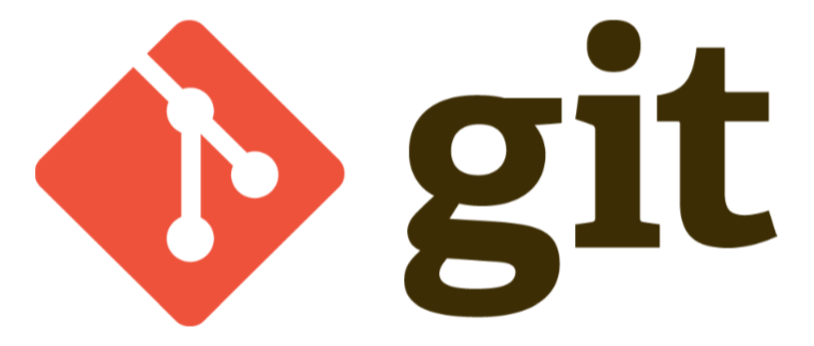
\includegraphics[width=0.2\textwidth]{img/git_logo.png}
  \caption{Git Versionsverwaltung \parencite[][]{Git:2016}}
  \label{fig:scrummodell}
\end{figure}

Bei DevOps werden alle in der Produktion entstandenen Artefakte an einer zentralen Stelle verwaltet. Dies geschieht in den meisten Fällen mit einer sogenannten Versionsverwaltung. Der Vorteil solcher Tools liegt darin, dass kollaborativ und ortstransparent an Artefakten gearbeitet werden und jegliche Änderungen genau dokumentiert werden. Somit befindet sich ein damit verwaltetes System immer in einem genau definierten Zustand. Es besteht auch die Möglichkeit, Änderungen ohne großen Aufwand rückgängig zu machen, oder unterschiedliche Versionen parallel zu verwalten.\\
Ein sehr bekannter Vertreter dieser Gattung von Tools ist Git. Es wurde entwickelt von Linus Torvalds, dem Erfinder von Linux, und hat sich mittlerweile zu einem sehr weit verbreiteten Versionsverwaltungstool entwickelt. Eines der Kernfeature ist die dezentrale Speicherung von Entwicklerrepositories, die es ermöglichen ortstransparent und effizient im Team zu kollaborieren. (NACHWEIS)

\begin{figure}[ht]
  \centering
  
\includegraphics[width=0.2\textwidth]{img/jenkins_logo.png}
  \caption{Jenkins Automatisierung \parencite[][]{Jenkins:2016}}
  \label{fig:scrummodell}
\end{figure}

Basierend auf dem Lean Prinzip der Optimierung, wird bei DevOps nicht nur die Organisation und Kollaboration optimiert, sondern auch auf technischer Ebene Entwicklung und Auslieferung. Als zentrales Element kommt hierbei oftmals eine Pipeline, in Form eines Continuous Integration Servers zum Einsatz. Eines der bekanntesten Open Source Projekte ist Jenkins. Dieses Projekt entstand aus dem Continuous Integration Server Projekt Hudson, nachdem dieses von Oracle aufgekauft wurde und viele Entwickler mit dessen Weiterentwicklung nicht mehr einverstanden waren. (NACHWEIS)\\
Ein Continuous Integration Server führt frei definierbare Aufgaben automatisiert aus und kann dabei mit unterschiedlichen Tools zusammenarbeiten. So kann er beispielsweise auf Änderungen in einer Versionsverwaltung reagieren und einen Bau- und Auslieferungsvorgang starten. Dabei können automatisierte Tests ausgeführt werden und das fertige Produkt auf verschiedene Systeme ausgeliefert werden. Die Einrichtung und Konfiguration solcher Continuous Delivery Server nimmt zu Beginn eines Projekts einige Zeit in Anspruch. Die zeitliche Ersparnis durch die vielen Möglichkeiten der Automatisierung gleichen diesen Aufwand aber wieder um ein Vielfaches aus. (NACHWEIS)\\
Continuous Integration Server bilden die Kerntechnologie bei DevOps, um eine schnelle Time To Market, schnelles Recovery nach Fehlerfällen, hohe Produktqualität und kurze Entwicklungszyklen zu erreichen.

\begin{figure}[ht]
  \centering
  
\includegraphics[width=0.2\textwidth]{img/chef_logo.png}
  \caption{Chef Konfigurationsverwaltung \parencite[][]{Chef:2016}}
  \label{fig:scrummodell}
\end{figure}

\begin{figure}[ht]
  \centering
  
\includegraphics[width=0.2\textwidth]{img/puppet_logo.png}
  \caption{Puppet Konfigurationsverwaltung \parencite[][]{Puppet:2016}}
  \label{fig:scrummodell}
\end{figure}

Ein weiteres Tool, welches Teil der Automatisierung ist und sehr gut mit einem Continuous Integration Server zusammen arbeitet ist eine Konfigurationsverwaltung. Diese Tools ermöglichen es, Konfigurationen zentral zu verwalten und automatisiert ablaufen zu lassen. Bei der manuellen Konfiguration von Servern und Systemen kommt es oft vor, dass sich Systeme in unterschiedlichen Zuständen befinden auf Grund unterschiedlicher Versionen, oder unterschiedlichen Herangehensweisen bei der Einrichtung. Dies bedeutet nicht nur bei der initialen Konfiguration, sondern auch bei allen darauf folgenden Updates und Upgrades einen erhöhten Zeitaufwand. Nicht standardisierte Systeme bedeuten auch im Fehlerfall einen erhöhten Aufwand bei der Suche und Beseitigung. Mit Hilfe von Konfigurationsverwaltungen erfolgt die Konfiguration aller System automatisiert, identisch und wiederholbar. Somit sinkt der Aufwand bei der initialen Konfiguration, bei Updates und Upgrades und im Falle eines Fehlers deutlich. Bekannteste Vertreter sind die Tools Chef und Puppet. Beide bieten eine sehr ähnlichen Grundfunktionalität, sind aber spezialisiert auf unterschiedliche Einsatzgebiete. (NACHWEIS)

\begin{figure}[ht]
  \centering
  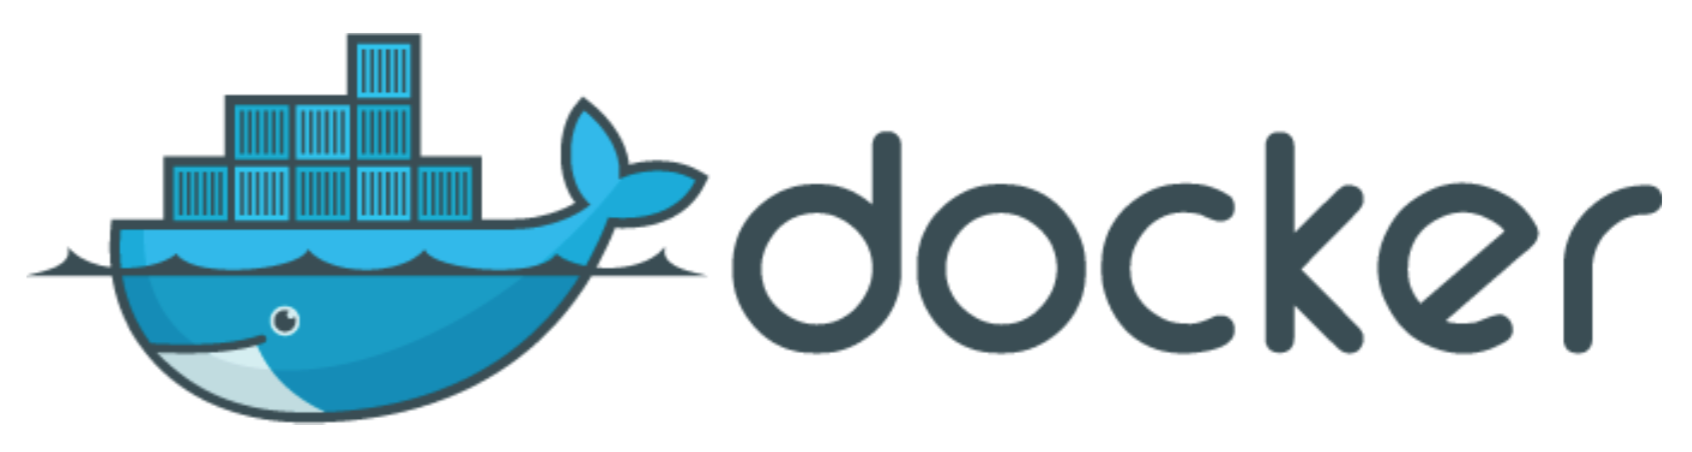
\includegraphics[width=0.2\textwidth]{img/docker_logo.png}
  \caption{Docker Deployment \parencite[][]{Docker:2016}}
  \label{fig:scrummodell}
\end{figure}

Das Deployment, oder Auslieferung, bildet das abschließende Element einer automatisierten Pipeline. Hier werden alle Produktionsartefakte zu einem lauffähigen System zusammengefasst und auf die entsprechende Infrastruktur ausgeliefert. Beispielsweise die Installation einer Shop Applikation auf einem Webserver. In diesem Bereich gab es in den letzten Jahren auf Grund steigender Performanz bei Hardware und Software große Sprünge in der Entwicklung. Dies führt dazu, dass Infrastruktur, beziehungsweise Plattformen virtualisiert werden können. Damit vereinfacht sich die Entwicklung und die Auslieferung um ein Vielfaches. Ein solches Tool zur Auslieferung und Virtualisierung ist Docker.\\
Docker ermöglicht es, ein System vollkommen identisch beliebig oft auszuliefern. Somit kann es bei der Auslieferung von Systemen keine Probleme mehr in Form von unterschiedlichen Konfigurationen, oder Installationen geben. Auch die Entwicklung profitiert von Virtualisierung, da so Betriebsumgebungen im Kleinformat zur Entwicklung genutzt werden können und es keine Unterschiede mehr zwischen Entwicklung und Betrieb gibt. Zudem erhöht Virtualisierung die Sicherheit, da einzelne Systeme vollständig getrennt auf dem selben Server arbeiten können und Angreifer nicht zwischen diesen wechseln können. (NACHWEIS)

\subsection{Kulturell}
Ein oft vergessener, aber durchaus wichtiger Teil von DevOps ist der kulturelle Aspekt. Um diesen genauer betrachten zu können müssen zuerst die unterschiedlichen Kulturformen einer Organisation erörtert werden.
Nach Westrum \parencite[Vgl.][]{Westrum:1988} gibt es drei unterschiedliche Arten von Organisationen:

\begin{itemize}
\item Machtorientierte Organisationen
\item Bürokratische Organisationen
\item Generative und Leistungsorientierte Organisationen
\end{itemize}

In machtorientierte Organisationen gibt es nur sehr wenig Kooperation und Kollaboration. Zudem wird Scheitern als sehr negativ angesehen und meist nicht akzeptiert. Mitarbeiter arbeiten nur für den eigenen Vorteil und versuchen sich selbst möglichst unentbehrlich darzustellen. In einer solchen Art der Organisation gibt es nur sehr geringe, oder gar keine Innovation, da Mitarbeiter nicht gewillt sind, Risiken einzugehen und neue Richtungen einzuschlagen.\\
Bürokratische Organisationen zeichnen sich dadurch aus, dass jede Abteilung und jeder Mitarbeiter genau definierte Aufgaben und Ziele haben. Von diesen wird nicht abgewichen, auch wenn sich dadurch ein Vorteil für einen Einzelnen, oder das Team entstehen würde. In dieser Art der Organisation herrscht oftmals Angst vor Veränderungen und Neuerungen, dementsprechend findet auch hier nur sehr geringen, oder aber gar keine Innovation statt. Kollaboration und Kooperation werden nur angewendet, wenn dies genau vorgegeben ist.\\
In generativen und leistungsorientierten Organisationen findet hingegen sehr viel Kooperation und Kollaboration statt. Es herrscht ein fehlerverzeihendes Umfeld, in dem Mitarbeiter dazu ermutigt werden, Risiken einzugehen und eventuell zu scheitern, da alle Mitarbeiter dadurch lernen können. Mitarbeiter arbeiten an einem gemeinsamen Ziel und teilen die dabei entstehenden Risiken, anstatt sie einzelnen Abteilungen, oder Personen zuzuschreiben. In einer solchen Organisation existiert keine Art der \glqq über die Mauer werfen\grqq Mentalität, bei der Probleme \glqq über die Mauer\grqq an andere Abteilungen weitergegeben werden, ohne diese zu lösen, um eigenen Ressourcen zu schonen. Jeder Mitarbeiter hat eine Verantwortung für die Qualität, die Verfügbarkeit und die Sicherheit des Produkts. Ein solches Umfeld fördert Innovation und das Beschreiten neuer Wege.\\
DevOps strebt eine generative und leistungsorientierte Organisationskultur an, bei der Mitarbeiter, besonders die der Abteilungen Entwicklung, Qualitätssicherung und Betrieb in hohem Maße kollaborieren und kommunizieren. Durch die Zusammenfügung verschiedener Abteilungen wird das Risiko auf alle Mitarbeiter gleichermaßen verteilt und alle sind für die Qualität des Produkts verantwortlich. Nur so lässt sich ein innovatives und effizientes Umfeld aufbauen, weshalb die kulturelle Ebene für DevOps von so großer Wichtigkeit ist.

\section{DevOps im Projektmanagement und ITIL} % 2 Seiten
Nachdem im vorangegangenen Abschnitt auf die praktische Umsetzung von DevOps eingegangen wurde, wird nun betrachtet, welche Anpassungen in Organisationen vorgenommen werden müssen, in denen andere Vorgehensmodelle eingesetzt werden und DevOps zum Einsatz kommen soll.

\subsection{Projektmanagement}
Um DevOps in einer Organisation einzusetzen, müssen entsprechende Anpassungen im Projektmanagement vorgenommen werden. Da DevOps keine Praktiken für Projektmanagement beinhaltet, kann hier auf bereits bestehende Vorgehensmodelle aufgebaut werden. Die umfangreichste Anpassung ist die Aufhebung der Trennung der Abteilungen der Entwicklung, der Qualitätssicherung und des Betriebs. Hierbei müssen die bestehenden Silos aufgelöst werden und ein gemeinsames Management für das gesamte Team geschaffen werden.\\
Bei der Projektplanung muss beim Einsatz von DevOps berücksichtigt werden, dass keine getrennten Phasen für Qualitätssicherung und Testen notwendig sind, sondern stattdessen Zeit für die Erstellung und Einbindung automatisierter Tests in die Entwicklungsphase eingeplant werden muss.\\
Durch den Einsatz von DevOps besteht zudem die Option, Fortschritt nicht nur in Textform als Bericht, sondern in Form lauffähiger Prototypen zu demonstrieren. Dies ist eine der wichtigsten Eigenschaften agiler Vorgehensmodelle, bei denen zum Sprint Ende, im Durchschnitt alle zwei Wochen, ein solcher Prototyp an den Kunde ausgeliefert wird. Mit Hilfe von DevOps ist es möglich, Prototypen mehrmals am Tag zu erzeugen. Mittels der automatisierten Pipeline entsteht aus jeder Änderung ein solcher Prototyp.\\
Ein weiterer Vorteil, den der Einsatz von DevOps mit sich bringt, ist das \glqq Design for Failure\grqq. In klassischen Projekten muss eine Fehlerstrategie extra erarbeitet werden. Bei DevOps besteht diese zum einen aus Standardisierung und Protokollierung jeglicher Änderungen, wodurch Fehlersuche sehr stark vereinfacht. Zum anderen besteht diese Strategie aus einem sehr schnellen Recovery, bedingt durch den hohen Grad an Automatisierung. Im Falle eines Fehlers, oder eines Ausfalls kann ein neues System automatisiert in kürzester Zeit neu ausgeliefert werden. Dies ist besonders bei cloudbasierten Diensten, oder Webapplikationen wie Online Shops von besonderer Bedeutung, da hier Ausfallzeiten besonders hohe finanzielle Auswirkungen haben. (NACHWEIS)

\subsection{ITIL}
ITIL ist im Bereich des IT Managements ein internationaler \glqq De-facto-Standard\grqq und findet daher in vielen IT Abteilungen Anwendung. Um DevOps in solch einem Umfeld einsetzen zu können, müssen keine vollkommen neuen Strukturen geschaffen werden, sondern DevOps kann parallel zu ITIL eingesetzt werden. Dies ist ein großer Vorteil von DevOps, da die Veränderung vorhandener Strukturen mit Kosten verbunden ist. So kann DevOps zunächst in geeigneten Bereichen getestet werden und bei Bedarf ausgebaut werden.\\
Zur Einführung von DevOps in ITIL orientierte Bereiche wurde folgende Vorgehensweise entwickelt:

\begin{itemize}
\item Identifizierung der ITIL Prozesse
\item Review der Prozesse
\item Identifizierung der Schwachstellen
\item Konkrete Planung
\item Priorisierung und Umsetzung
\end{itemize}

(NACHWEIS)

Zunächst werden geeignete Bereiche im entsprechenden Umfeld identifiziert, in denen ein ausreichend großer Vorteil durch Automatisierung und verbesserte Zusammenarbeit entstehen kann. Daraufhin werden die wichtigsten ITIL Prozesse in diesen Bereichen identifiziert. Nach diesem Schritt werden die ausgewählten ITIL Prozesse einem Review unterzogen. Dieser findet mit allen an diesen Prozessen beteiligten Abteilungen statt. Nur so kann sichergestellt werden, dass der Einsatz von DevOps an dieser Stelle optimal und ohne Verlust ist. Um den Aufwand und die Dauer hierbei in Grenzen zu halten, können diese Reviews als Workshop veranstaltet werden. Auf das Review folgt nun die Identifizierung der Schwachstellen der jeweiligen ITIL Prozesse. Hierbei liegt der Fokus darauf, welche Fehler den höchsten Schaden verursachen können. Dabei werden die Eintrittswahrscheinlichkeit und die Kosten im Falle eines Fehlers untersucht. Anschließend werden konkrete Maßnahmen definiert, wie in diesen Prozessen Automatisierung und Kollaboration gewinnbringend eingesetzt werden können. Dies geschieht nun auf einem niedrigeren Abstraktionsniveau und liefert als Ergebnis die tatsächlich geplante Umsetzung. In einem letzten Schritt folgt eine Priorisierung der einzelnen ITIL Prozesse und Maßnahmen und die tatsächliche Umsetzung.


\section{Optimierungspotentiale und Verbreitung} % 1 Seiten

\subsection{Optimierungspotentiale}
Gartner
Einsatz verstärkt in Cloud und Mobile Branchen
IT-Führungskräfte befragt
Was hat Einführung von DevOps gebracht?
Schnellere Time to Market
Wiederverwendung / Automatisierung: Risikominimierung, Einsparung von Entwicklungsaufwand

\subsection{Verbreitung}
... siehe Bubbles


\section{Aktuelle Entwicklung von DevOps} % 3 Seiten
Bisher:
Nicht Teil des automatisierten Prozesses
Auf Entwicklung folgendes “Bottleneck”

\subsection{DevOps und Sicherheit}
Integration von Sicherheit in Pipeline: automatisierte Sicherheitstests

keine manuellen Änderungen am System (Überschreiben)
keine Updates -> nur Upgrades (neue Version)
Phoenix Upgrades / Blue-Green Upgrades

Immutable Infrastructure / Wegwerf Infrastruktur
Trennung von Daten und Infrastruktur (Rechte)

Auditierung und Compliance vereinfacht
- vereinfacht
- alles zentral und versioniert
- alle Änderungen protokolliert
- genau definierter Zustand
- Compliance Tests in Pipeline

Security as Software
- Vision
- komplette Sicherheit in Pipeline
- Automatisierung nicht einfach
- erfordert gewisse Abstraktion


\section{Fallstudie} % 3 Seiten
Nordstrom Fashion Retailer

\subsection{Einführung}
getrennte Abteilungen
lange Update Zyklen
langsame Reaktion auf Probleme
Homepage Upgrade (über Nacht, Ausfallzeiten)
Kassensystem Server Upgrade (Lange Dauer, Vor-Ort-Einsatz)

\subsection{Optimierungspotentiale durch DevOps}
in kleinem Bereich
Bezahlsysteme in den Läden
Virtualisierung der Bezahlsysteme
Virtualisierung -> einfaches Deployment (keine Arbeit vor Ort)
Windows Server 2003

Einsparung von Arbeitszeit und Aufwand
Kürzere Ausfallzeiten
schnellere Recovery

\subsection{Durchführung und Ergebnis}
Entwickler der Server, Datenbank, Website
Operations Leute, die vor Ort arbeiten

einige Wochen Arbeit
vollautomatisierte Erstellung in 4h statt 18h Arbeit vor Ort
Wiederholbar
Tests in Entwicklung
Entwicklung an original Systemen
Erfahrungen gesammelt, um Entwicklung des Herzstücks, der Homepage, zu automatisieren
